%%%%%%%%%%% ESTADO DEL ARTE    %%%%%%%%%%
\chapter{Estado del Arte\label{ch:EstadoDelArte}}

En este Capítulo se presenta el estado del arte de los sistemas \Gls{ABC} en la Sección \ref{sec:estadoArteABC}. En la sección \ref{sec:estadoArteAtaquesPresentacion} de los ataques de presentación y específicamente, de los ataques de presentación con \gls{morphing} en la sección \ref{sec:estadoArteMorphing}.

%%%%%%% ESTADO DEL ARTE DE LOS SISTEMAS ABC %%%%%%%%%%%%
\section{Sistemas ABC}\label{sec:estadoArteABC}

Los \GLS{ABC} son sistemas multi-sensor con tres tareas principales: Primero, digitalizar la documentación del viajero y autentificar su validez. Después, comprobar que el viajero es quien dice ser, mediante una verificación biométrica entre los rasgos del viajero y los almacenados en los documentos (comúnmente rasgos faciales y dactilares). Y finamente, comprobar si el viajero tiene derecho a cruzar la frontera. según las normas administrativas y legales. Algunos sistemas \cite{didier2015eu} \cite{anand2016enhancing} \cite{del2016automated} \cite{Gorodnichy2015ARTinABC} separan en estas tareas en dos etapas: Una etapa de registro (\GLS{RTP}, \textit{Register Traveller Programme}) y otra de validación (\GLS{EES}, \textit{Entry/Exit System}). En el registro, se auténtica documentación y se comprueba la idoneidad para cruzar la frontera, mientras que la verificación biométrica, se realiza en la validación. En ocasiones. estás dos etapas lógicas se separan físicamente en dos dispositivos, dando lugar a una topología de \GLS{ABC} segregada \cite{del2016automated}.

\begin{figure}[t]
    \centering
    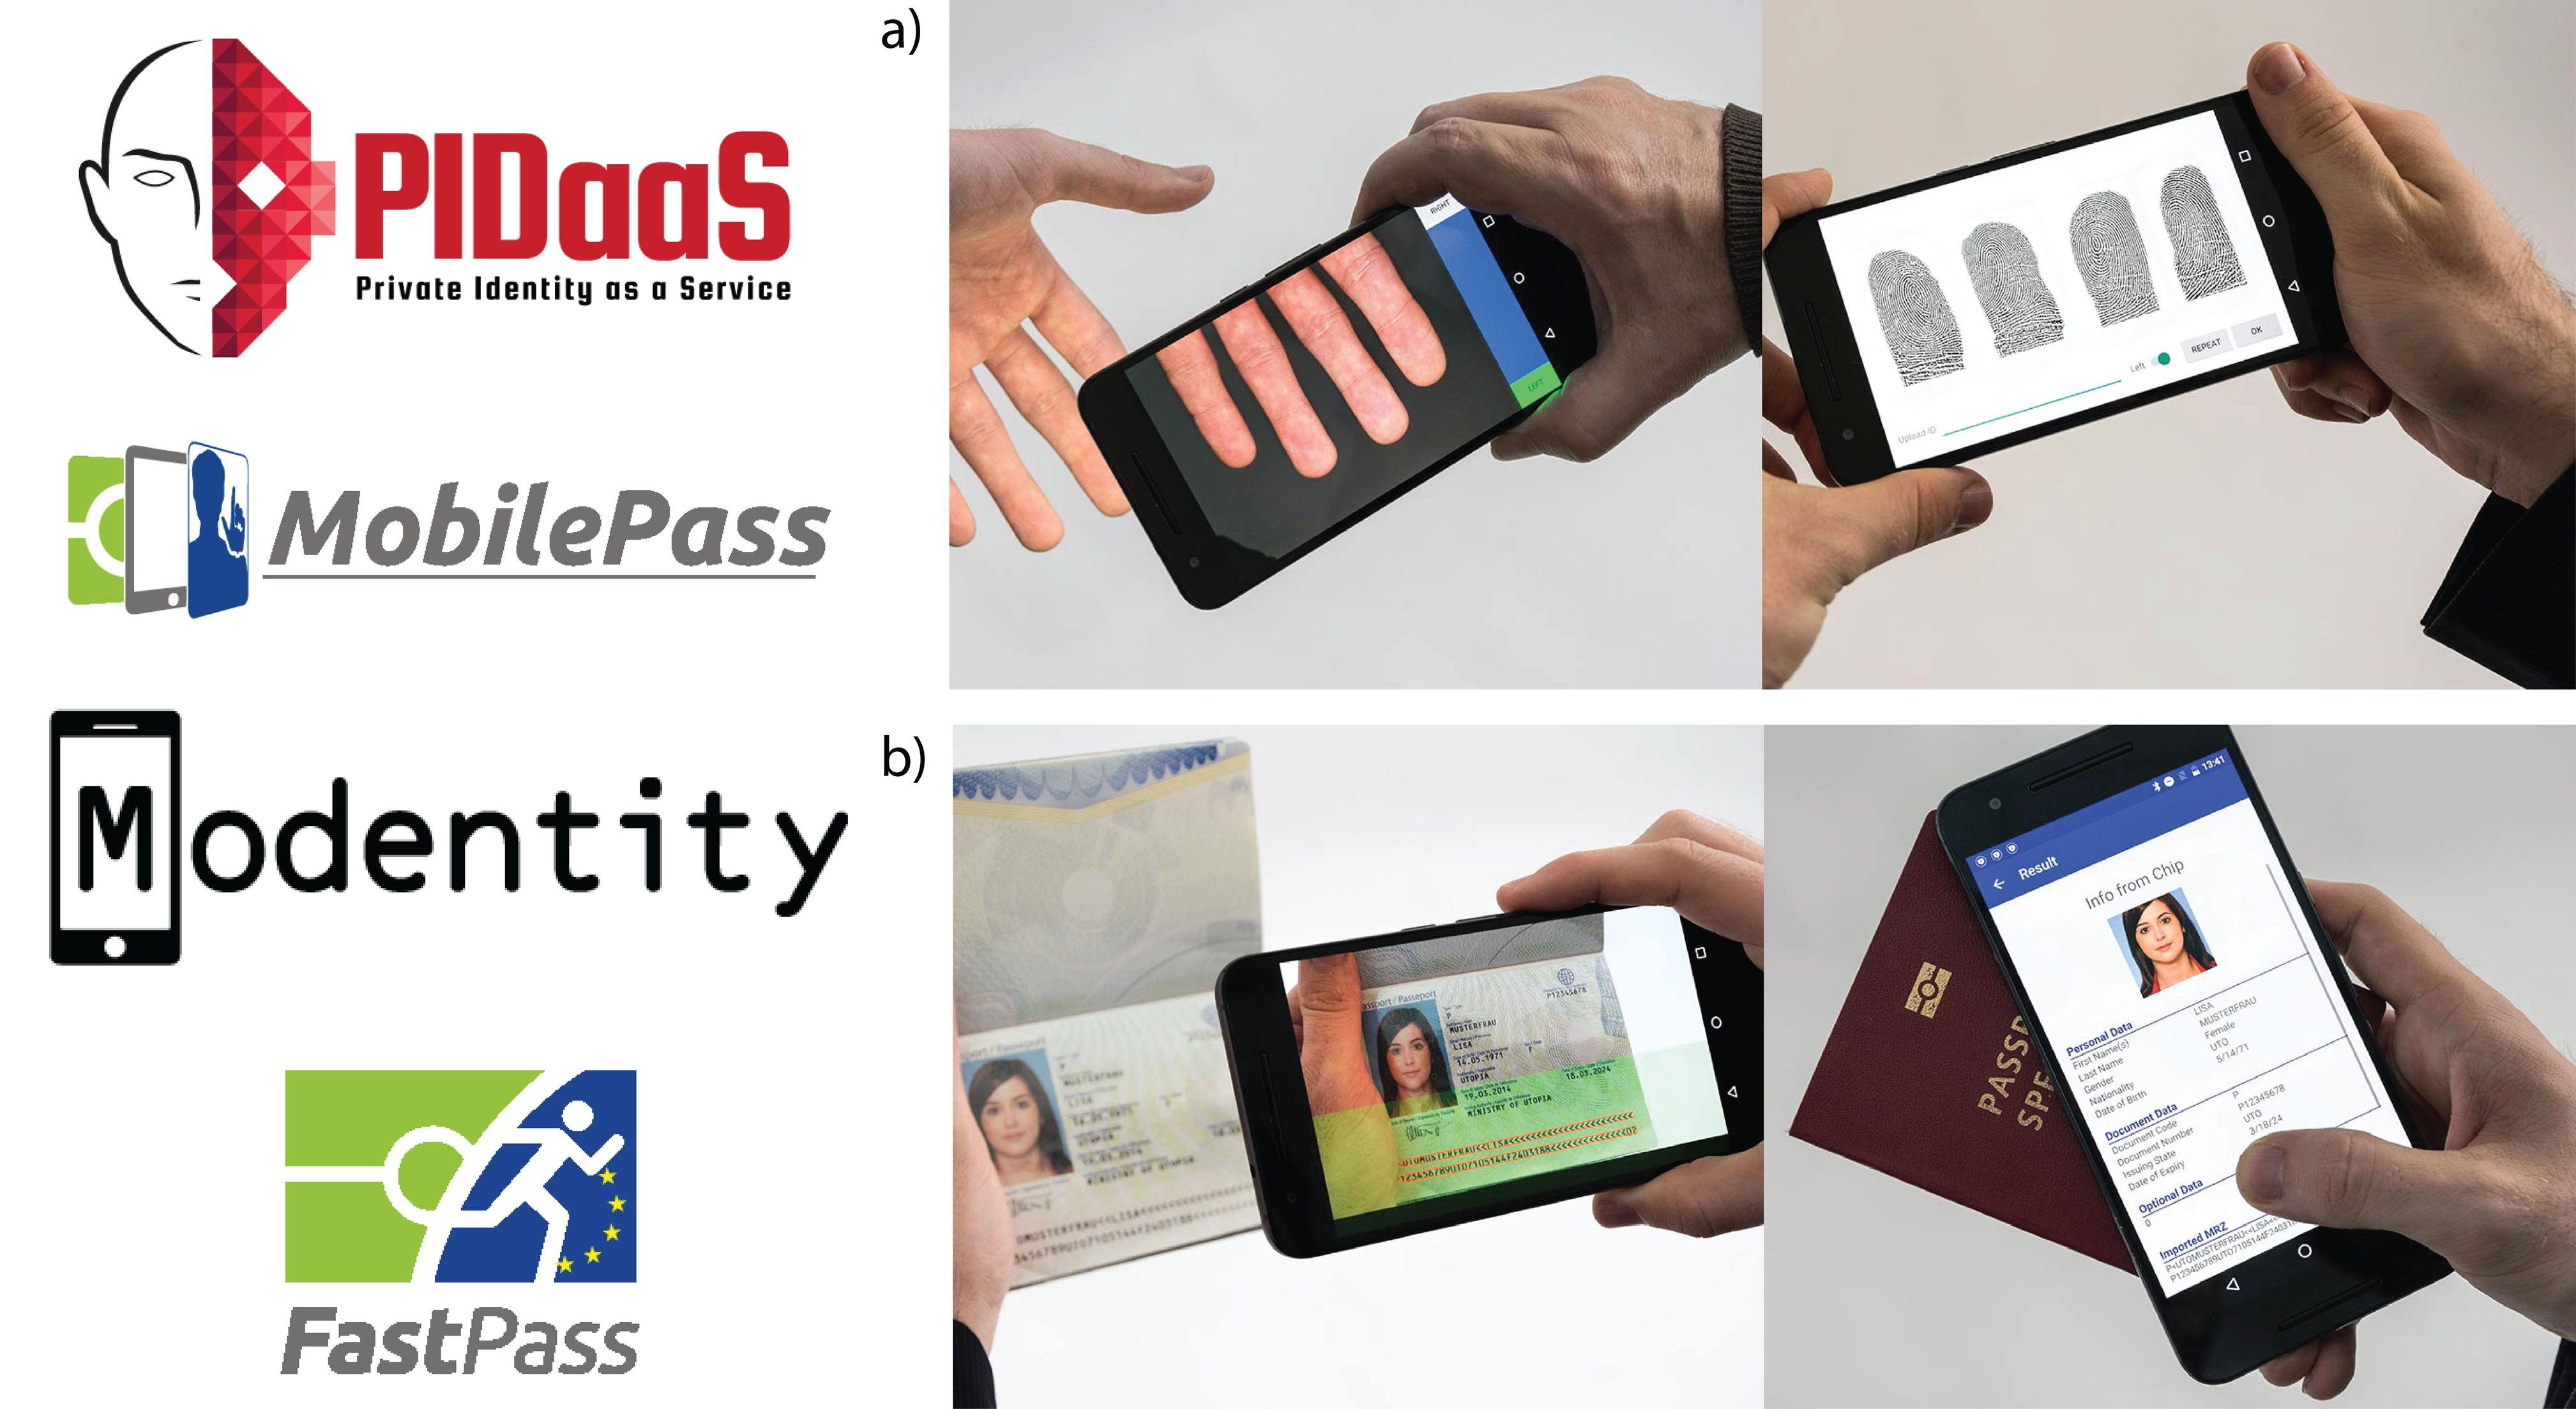
\includegraphics[width=0.9\textwidth]{ch-sistemasABC/images/ch-SistemasABC/CAPTURA_MOBIL_Y_PROYECTOS.png}
    \caption{A la izquierda Proyectos de investigación y empresas dedicados a sistemas móviles: \Gls{MobilePass}\cite{MobilePassOnline}, \Gls{Modentity}\cite{ModentityOnline}, \Gls{PIDaaS}\cite{PIDaaSOnline}. Y a la derecha, funcionalidades de los sistemas \GLS{ABC} móviles del proyecto \gls{Modentity} \cite{ModentityOnline}. a) Verificación dactilar sin contacto y b) Digitalizado y lectura \GLS{NFC} de un pasaporte}
    \label{fig:modentityFunciones}
\end{figure}

\begin{figure}[t]
    \centering
    
\includegraphics[width=0.8\textwidth]{ch-sistemasABC/images/ch-SistemasABC/LOGOS_EMPRESAS.png}
    \caption{Empresas dedicadas a sistemas \GLS{ABC}:\Gls{MODI} \cite{MODIOnline}, \Gls{INDRA} \cite{indraOnline}, \Gls{VisionBox} \cite{visionBoxOnline}, \Gls{Gemalto} \cite{gemaltoOnline}, \Gls{ARH} \cite{ARHOnline},\Gls{Innovative} \cite{InnovativeOnline}}
    \label{fig:logosEmpresasABC}
\end{figure}

Para su homologación, los sistemas \GLS{ABC}, deben ajustarse a la legislación de fronteras de cada país, por ejemplo al \GLS{SBC} \cite{SBCode2016} en \GLS{EU}. Y también, satisfacer ciertos estándares internacionales cómo los fijados para sistemas biométricos de \GLS{ISO}/\GLS{IEC} $19794$ \cite{ISO/Biometric} o los de uso de documentos \gls{eMRTD} de \GLS{ICAO} Doc $9303$ \cite{doc20069303}. Del mismo modo es conveniente que tengan en cuenta las recomendaciones técnicas \cite{FRONTEX2016TechReport} y operativas \cite{FRONTEX2016OpeReport}, presentadas por \Gls{frontex} \cite{FRONTEXOnLine}. 

El subsistemas biométrico es un componente fundamental en los \GLS{ABC} \cite{labati2016biometric} \cite{spreeuwers2012evaluation}. Es posible encontrar sistemas que hacen uso de diferente rasgos biométricos: huellas dactilares \cite{anand2016enhancing} \cite{gamassi2005robust}, la cara \cite{del2015face} \cite{del2016automated} \cite{kosmerlj2006face}, el iris \cite{daugman2015iris} \cite{palmer2012ten} \cite{matey2006iris}, e incluso sistemas con biometría palmar (geometría de la mano) \cite{nanavati2011biometric}. Pero la tendencia es usar sistemas multi-biométricos \cite{cantarero2013multi} \cite{cimato2006personal} \cite{cimato2008privacy} \cite{gamassi2004high} \cite{gamassi2005multi}.

% %BIOMETRIA DEL IRIS EN LOS SISTEMAS DE ABC DE CRUCE DE FRONTERAS
% @article{daugman2015iris,

% %PRESENTA LOS PROBLEMAS DE LA BIOMETREIA DEL IRIS EN LOS SITEMAS ABC
% palmer2012ten,

% %RECOCIMIENTO DEL IRIS EN MOVIMIENTO 
% matey2006iris

Los sistemas \GLS{ABC} están en continua evolución, asimilando tecnologías emergentes y nuevos desarrollos. Muchas instituciones gubernamentales, nacionales e internacionales, gestionan proyectos de investigación dedicados este tipo de sistemas, como: \GLS{ABC4EU} \cite{ABC4EUOnline}, \Gls{FastPass} \cite{FastPassOnline}, \cite{berglund2008frontex} o \cite{kosmerlj2006face}. También en el sector privado, muchas empresas se dedican a la investigación y al desarrollo de este tipo de sistemas: \Gls{MODI} \cite{MODIOnline}, \Gls{INDRA} \cite{indraOnline}, \Gls{VisionBox} \cite{visionBoxOnline}, \Gls{Gemalto} \cite{gemaltoOnline}, \Gls{ARH} \cite{ARHOnline}, \Gls{Innovative} \cite{InnovativeOnline}. Y otras como: \Gls{Cognitec} \cite{cognitec2019url} o \Gls{Dermalog} \cite{DermalogOnline} proporcionan desarrollos cruciales para el subsistemas biométricos de los \GLS{ABC}.     

% En el caso de los cruces de frontera europeos en los que se utilizan sistemas \GLS{ABC}, se requiere comprobar la identificación del sujeto con dos listas: \GLS{RTP} (\textit{Register Traveller Programme}) y \GLS{EES} (\textit{Entry/Exit System}) \cite{didier2015eu}. La identidad de los viajeros y su idoneidad para cruzar la frontera se verifica en el control del \GLS{RTP} según la información almacenada en su documentación. Una vez identificados los viajeros, se registran sus datos. En el momento de cruzar la frontera, el \GLS{EES} obtiene la coincidencia biométrica entre la información registrada y los datos capturados.

% Dependiendo de los dispositivos en los que se realizan los procesos de \GLS{RTP} y \GLS{EES}, hay diferentes topologías de sistemas \GLS{ABC}: Proceso de un paso y proceso de dos pasos \cite{anand2016enhancing}. En la topología del proceso de un solo paso, la \GLS{RTP} y el \GLS{EES} se fusionan en un solo proceso en el que la identificación de los viajeros se lleva a cabo al mismo tiempo que éstos cruzan la frontera. Los dispositivos para este tipo de topología suelen ser trampas electrónicas \cite{del2016automated}, que no permiten el cruce hasta que la identificación se haya realizado correctamente. En la topología de proceso en dos etapas, los procesos \GLS{RTP} y \gls{EES} están bien diferenciados. Primero, se registran los viajeros y luego, su información biométrica se compara antes de permitir el cruce. Se puede considerar que el \GLS{ABC} de dos pasos integrado o segregado atiende si el\GLS{RTP} y el \GLS{EES} se logran a través de uno o dos dispositivos. 

% En cuanto a la implantación de los sistemas \GLS{ABC} y su utilidad, es importante mencionar que casi todos los aeropuertos que reciben viajeros de países no pertenecientes a \Gls{Schengen} los utilizan (un mapa completo de los aeropuertos con \GLS{ABC} se presenta en \cite{iata2018abc}). Sin embargo, los puertos marítimos equipados con \GLS{ABC} no son tan comunes. 

% Los sistemas \GLS{ABC} pueden tener varias configuraciones físicas \cite{morosan2018information}. Las más típicas utilizan puertas electrónicas (\gls{e-gate}) \cite{donida2016emerging}. Estos dispositivos regulan el flujo de viajeros a través de la frontera mediante el uso de sensores biométricos (por ejemplo, cámaras de reconocimiento facial \cite{labati2016biometric} y lectores de huellas dactilares \cite{anand2016enhancing}, lectores de documentos de viaje (por ejemplo, escáneres \cite{nguon2017system} y lectores de chip sin contacto por radiofrecuencia \cite{abdal2016authentication}, así como barreras físicas que permiten (o no) al viajero cruzar la puerta electrónica \cite{nieto2014walls}.

% Profundizar en el diseño de los sistemas \GLS{ABC}, su capacidad para volver a cubrirse de situaciones problemáticas (es decir, la resistencia) y para resistir ataques externos (es decir, la robustez) son sus principales requisitos de seguridad. La mayoría de los ataques típicos se centran en el sistema biométrico. Estos ataques se denominan ataques de presentación, que consisten en que un atacante presenta características biométricas falsificadas de otro sujeto a los sensores para obtener permiso para cruzar la frontera. Por esta razón, los sistemas \GLS{ABC} incluyen algún tipo de \GLS{PAD} y módulo \GLS{PAD} en el proceso de reconocimiento biométrico. 

% Los sistemas \GLS{ABC} hacen uso de puertas electrónicas (\gls{e-gate}), que son dispositivos para controlar de forma automática el flujo de viajeros que cruzan la frontera por medio de elementos móviles o fijos, escáneres para la lectura de documentos y sensores para realizar captura biométrica. En particular, el viajero  presenta su \gls{eMRTD} al escáner del sistema, que detecta y extrae sus datos personales de la llamada zona de lectura mecánica \GLS{MRZ} del documento (figura \color{red} Alguien en el registro, en el paper era una de Cristina\color{cyan}). Una consulta a la base de datos de cruces permitidos viajero se hace y luego, si se tiene éxito, el los datos biométricos del viajero se extraen del chip del documento. Estos datos pueden incluir un conjunto de fotos faciales, huellas dactilares, etc. El viajero entonces tiene que proveer al sistema \GLS{ABC} con su sistema biométrico características en ese mismo momento (\gls{vivo}), que se comparan con los que se leen en el chip del documento. Si es una coincidencia, entonces la puerta electrónica abre las puertas y se permite a los viajero cruzar la frontera.

% Existen tres configuraciones posibles para un sistema \GLS{ABC} (Ver Fig. \ref{fig:TopologiasABC}): Primero, un viajero a la vez se hace entrar en una trampa, que es un cubículo con dos puertas. En este espacio, tanto la autenticación del documento y la verificación biométrica se hacen en paralelo en un proceso de un solo paso, por lo que esta solución puede ser muy rápida. Las otras dos configuraciones utilizan un proceso de dos pasos. Por un lado, la solución integrada, en la que la autenticación de los documentos tiene lugar justo fuera de un Figura \color{red}ESTA ES LA IMAGEN DE CRISTINA EN EL REGISTRO DE BARAJAS\color{cyan}: Ejemplo de un \GLS{ABC}. Foto tomada del piloto experiencia en el Aeropuerto Adolfo Suárez Madrid-Barajas T$4$-$S$ terminal de llegadas internacionales \cite{aeropuertoMadridBarajas}, \gls{mantrap}, dentro de la cual se lleva a cabo la captura biométrica.

% En una tercera configuración, la solución segregada, la autenticación de documentos y la biométrica la verificación se realiza en un quiosco de inscripción, mientras que se hace una segunda verificación biométrica en la puerta única \gls{e-gate}.

% Para más información sobre el \GLS{ABC}, el lector puede revisar \cite{labati2016biometric}, que proporciona un estudio sobre el reconocimiento biométrico en los sistemas \GLS{ABC}, mientras que \cite{del2015face}, se centra específicamente en sistemas \GLS{ABC} basados en el reconocimiento facial.
% \color{black}

\color{red}
Ver cronología de publicaciones sobre los sistemas \GLS{ABC} (Apéndice \ref{apendix:ApendiceCronologiaABC})

Ver cronología de publicaciones sobre \gls{biometria} (Apéndice  \ref{apendix:ApendiceCronologiaBiometria})
\color{black}

%%%%%%% ESTADO DEL ARTE DE LOS ATAQUES DE PRESENTACION %%%%%%%%%%%%%%%%%%%%%%%%
\section{Ataques de presentación}\label{sec:estadoArteAtaquesPresentacion}

El sistemas biométrico de los \GLS{ABC} puede ser atacado en diferentes etapas\footnote{\GLS{ISO}/\GLS{IEC} $30137$-$1$:$2019$ -  Part 1: System design and specification \cite{ISO/Biometric}}: en el sensor, en la base de datos, en las comunicaciones, o el modulo de proceso, etc.. Los ataques de presentación tienen lugar en el dispositivo en la fase de captura del sistema \cite{ratha2001enhancing}.

Una primera clasificación\footnote{\GLS{ISO}/\GLS{IEC} $30107$-$1$:$2016$ Biometric presentation attack detection — Part 1: Framework  \cite{ISO/PADFramework}} de estos ataques incluye: los ataques con base documental que requieren de la manipulación de los documentos de viaje: falsificaciones \cite{tolosana2019presentation} o \gls{morphing}  \cite{scherhag2018towards}), y de base biométrica que se basan en la suplantación (\gls{spoofing}) de los rasgos biométricos del viajero por parte del atacante.

Cuando el viajero proporciona sus características biométricas voluntariamente e interactúa con el sistema de la manera esperada, la presentación  se considera una presentación \gls{bona-fide}. Pero, cuando una persona trata de interferir con el funcionamiento normal del sistema, se considera un \GLS{PA}. El rasgo u artefacto utilizado en el ataque se llama \textit{Presentation Attack Instrument} (\GLS{PAI}). Existen distintos tipos de \GLS{PAI} (\GLS{ISO}/\GLS{IEC}, $2016$b \cite{ISO/PADFramework}): Una fotografía (impresa en papel \cite{scherhag2017vulnerability} \cite{rigas2015eye} \cite{anjos2011counter} o reproducida en una pantalla \cite{li2016generalized}), una máscara de cartón \cite{del2017face}, de silicona \cite{bhattacharjee2018spoofing} \cite{manjani2017detecting} o impresa en $3$D \cite{agarwal2017face}, una huella sintética \cite{sousedik2014presentation}, una imagen de alta resolución de iris \cite{raja2016color} o incluso el verdadero dedo de un cadáver \cite{deadFinger}.

Los \GLS{PAD} son métodos para la detección ataques de presentación \cite{marcel2014handbook}. Pueden ser métodos hardware o software.
Los métodos hardware se apoyan en el sensor y se basan en propiedades intrínsecas, como el pulso o el parpadeo de los individuos \cite{rigas2015eye}. En algunos casos el sistema produce un estímulo y espera una respuesta del viajero {\gls{challenge response}} \cite{shoukry2015pycra}.
Entre los métodos \textit{software} existen distintos enfoques en la literatura: Basados en micro-texturas, basados en la deformación de  los rasgos biométricos, basado en la búsqueda de artefactos, basado en la imagen espectral y enfoques híbridos.
Algunos de estos enfoques se basan en características temporales por lo que necesitan una captura de vídeo. 


% \cite{ramachandra2017presentation}. Los métodos basados en hardware (o a nivel de sensor) se basan en las propiedades intrínsecas del cuerpo. Nótese que, en algunos casos, se necesita un sensor específico o no convencional para adquirir estas características. Ejemplos de estas propiedades son: texturas faciales, resistencia eléctrica, temperatura, sudor, color, resistencia de la piel a otras longitudes de onda no visibles y forma tridimensional. Algunas de estas propiedades son involuntarias, ya que están controladas por el sistema nervioso, en particular el pulso, las sacadas oculares y la respiración. En el caso de los sistemas \GLS{PAD}, producen un estímulo y tratan de detectar las reacciones del cuerpo (métodos de desafío-respuesta) \cite{shoukry2015pycra}. Un ejemplo común de estos métodos es pedir al usuario que siga una luz con la cabeza, o que lea en voz alta una frase. Se pueden buscar reacciones involuntarias como el parpadeo de los ojos o la constricción de la pupila debido a la luz deslumbrante \cite{rigas2015eye}. Aunque estas tareas se pueden realizar por medio de software, también se pueden realizar por medio de hardware dedicado. Por último, el uso de estrategias multi-modales (mismo rasgo, múltiples sensores) o multi-biométricas (múltiples rasgos, mismo sensor) puede aumentar la robustez del sistema contra los ataques de suplantación de identidad

% Por el contrario, los métodos basados en software (o basados en rasgos) son capturados por un módulo situado justo después del sensor, funcionando así con la muestra biométrica adquirida. Esto proporciona una gran precisión y un costo relativamente bajo \cite{ramachandra2017presentation}. La mayoría de estos métodos sólo se basan en características estáticas (es decir, en una sola imagen). Estos últimos pueden organizarse en métodos estáticos basados en texturas y métodos estáticos basados en frecuencias \cite{ramachandra2017presentation}. Los métodos basados en texturas pueden detectar rasgos faciales o incluso la presencia de artefactos debido a la mala calidad de impresión. Los métodos basados en la frecuencia utilizan la información espectral contenida en una imagen facial. Ambos métodos pueden combinarse utilizando enfoques híbridos. Sin embargo, algunos métodos basados en el software son dinámicos en el sentido de que también tienen en cuenta la información temporal. Por ejemplo, cuando el sensor adquiere vídeos en lugar de instantáneas. Por lo tanto, algunos métodos basados en la textura dependen de las características de movimiento de los datos entrantes, como el seguimiento del movimiento de la cabeza, el movimiento de fondo o el flujo óptico \cite{tiwari2016dynamic}.

% Centrándose en los \GLS{PA} de \gls{biometria} facial, en la literatura se pueden encontrar estudios sobre módulos \GLS{PAD} para diferentes \GLS{PAI} \cite{hernandez2019introduction}. Por ejemplo, los llamados foto-ataques consisten en presentar una imagen de la cara al sistema en lugar de la cara misma \cite{rigas2015eye} \cite{anjos2011counter}. Esta imagen puede ser una fotografía estándar impresa en papel o puede mostrarse con la ayuda de dispositivos electrónicos (ordenador portátil, tableta o teléfono móvil). Estos dispositivos pueden mejorar el ataque mostrando un vídeo delante del sensor\cite{li2016generalized}. Este sensor normalmente sólo tiene en cuenta el movimiento normal de la cabeza o características específicas como los labios (al leer una frase) o los ojos (parpadeo, reacción a la luz), lo que dificulta la detección del ataque. Este problema puede resolverse detectando la presencia de algunos elementos extraños como las manos en la imagen adquirida o en los bordes de la imagen. Otro tipo de ataque bien conocido es el que utiliza máscaras faciales \cite{manjani2017detecting}. El caso más fácil es imprimir una foto de la cara en una máscara que es utilizada por el atacante. La zona de los ojos suele estar cortada a al- bajo los ojos del atacante para que sea visible y así evitar un posible módulo de detección de parpadeo \cite{bhattacharjee2018spoofing}. Por otra parte, la llegada de impresoras $3$D baratas ha allanado el camino para la creación de máscaras $3$D realistas que imitan los rostros de otros individuos \cite{agarwal2017face}. Existen varias soluciones comerciales para crear estas máscaras con un puñado de fotografías normales (de frente y de dos lados). También en este punto es importante considerar el uso de maquillaje facial, disfraces, pelucas, barbas o bigotes falsos, e incluso la cirugía plástica para llevar a cabo este tipo de ataques de presentación \cite{chen2016unconstrained}. 

% Los ataques de presentación pueden clasificarse en dos. Primero, los ataques de presentación que hacen uso de los auténticos rasgos humanos, incluyendo partes de un cuerpo muerto, características físicas intencionalmente modificado (cicatrices, cirugía, cambios temporales inducidos por medicación), la suplantación de la personalidad de otra persona coincidencia accidental de la característica de otra persona en una presentación de \gls{bona-fide} (impostor de esfuerzo cero tentativa), o presentación de características genuinas obtenidas bajo coacción o amenaza.

% Un segundo tipo de ataques de presentación emplean \GLS{PAI} artificiales. Artefactos que pueden obtenerse directamente de la característica biométrica real, por ejemplo con un molde, o de forma indirecta de una muestra latente, como una huella dactilar dejada en una superficie. El rasgo biométrico también puede ser robado mediante  un dispositivo de grabación, como cámara de vídeo o una cámara fotográfica.

% Características completamente sintéticas generadas sin semejanza con las características de un usuario específico puede ser consideras también como un ataque de presentación.

% PAD, Existen distintos tipos: comprobación de la vida \cite{bhattacharjee2018spoofing}, esto es, la comprobación de que el rasgo biométrico se está adquiriendo de una persona viva. Por ejemplos mediante la medición de la temperatura corporal, la detección de los vasos sanguíneos o el parpadeo de los ojos.

% Existen varias técnicas para llevar a cabo tales ataques, pero todas ellas pueden organizarse en ataques de base biológica y ataques de base documental \cite{tolosana2019presentation}. Los primeros se centran principalmente en tres elementos principales: el rostro \cite{scherhag2017vulnerability}, la huella dactilar \cite{sousedik2014presentation} y la huella ocular (es decir, el reconocimiento del iris) \cite{raja2016color}. Este último suele considerar los documentos utilizados por los viajeros para identificarlos (por ejemplo, pasaporte y otros documentos de viaje) \cite{kraetzer2017modeling}. Es típico que estas chinchetas puedan abordar más de un elemento (por ejemplo, la cara y la aleta de la huella, o la cara en la foto del pasaporte \cite{scherhag2018towards}).


% \subsubsection{PAD. Detección de ataques de presentación} %%%%%%%%%%% ETADO DEL ARTE PAD

% El reconocimiento facial automático ha alcanzado altas tasas de rendimiento \cite{zhao2003face} \cite{jain2011handbook}, especialmente desde la aparición del \textit{deep learning} \cite{schroff2015facenet} \cite{parkhi2015deep} y esto ha hecho que se hayan multiplicado el número de aplicaciones que hacen uso de biometría facial.

% Los sistemas biométricos, incluidos los basados en el reconocimiento facial, suelen comprender varios módulos dedicados a funciones específicas, como la captura de datos (sensor), la extracción de características, el almacenamiento de datos, la comparación de puntuaciones y la toma de decisiones (para la normalización, \cite{ISO/Biometric}). Según el módulo del sistema que se piratee, pueden identificarse varias vulnerabilidades. En particular, los ataques de presentación tienen lugar en el extremo frontal del sistema (es decir, a nivel de los sensores). Así, los atacantes presentan el sistema con rasgos biométricos falsos (es decir, falsos o falsificados). Estos tipos de ataques son fáciles de cometer ya que son externos al sistema, a diferencia de otros que requieren un conocimiento profundo del funcionamiento del sistema (por ejemplo, para piratear el extractor de características, la base de datos, la clasificación o los módulos de decisión). Esta cuestión hace que los ataques de presentación sean la forma de ataque más probable para un sistema de reconocimiento de rostros \cite{marcel2014handbook}. 

% En el caso de \GLS{FlyPAD}, la tarea de \GLS{PAD} depende de algoritmos basados en hardware. Estos algoritmos son capaces de detectar individuos distantes, indicando posibles ataques de presentación mientras están en movimiento (es decir, sobre la marcha). Esta cuestión difiere de la literatura conexa sobre el tema, ya que es una de las principales novedades que ofrece el sistema. 

%%%%% ESTADO DEL ARTE DEL MORPHING %%%%%%%%%%
\section{Morphing}\label{sec:estadoArteMorphing}

El \gls{morphing} \cite{ferrara2014magic} es otro tipo de ataques que afecta a los sistemas \GLS{ABC}, donde los rasgos biométricos del viajero y los del atacante se combinan para producir un rasgo intermedio. que se almacena en el \Gls{eMRTD} y permite engañar al sistema.

El rasgo biométrico más empleado para ataques con \gls{morphing} es la cara , pero puede realizarse con otro tipo de rasgos como el \gls{iris} \cite{rathgeb2017feasibility} o la huella \gls{dactilar} \cite{ferrara2016feasibility}. 

El proceso de \gls{morphing} puede realizarse manualmente mediante programas especializados (\GLS{GAP}-\GLS{Gimp} \cite{GimpOnline}) \cite{raghavendra2016Detecting} , \cite{scherhag2017vulnerability}, \cite{ferrara2017face}, \cite{ferrara2018face}, pero en la literatura el método más empleado se basa en el algoritmo de triangulación \textit{Delaunay-Voronoi} (\GLS{DVT}) \cite{scherhag2018towards}, \cite{scherhag2018morph}, \cite{scherhag2018performance}, \cite{spreeuwers2018towards}, \cite{debiasi2018prnu}, \cite{debiasi2018prnuvar}. Algunos estudios como \cite{damer2018morgan} \cite{peng2019fd}, y en algunos casos realizando una mejora en resultado final para objetr una mejor calidad visual \cite{kraetzer2017modeling}, \cite{zhang2018face}, \cite{makrushin2017automatic}, \cite{seibold2018reflection}, \cite{seibold2018accurate}, \cite{wandzik2018morphing}, también realizan, fusión de las caras mediante \textit{Convolutional neural network} \GLS{CNN} arquitectura \GLS{GAN} \cite{damer2018morgan}. 

Los métodos \GLS{PAD} específicos para ataques de morphing se conocen como \textit{Morphing Attack Detection} (\GLS{MAD}). Existen dos tipos de métodos \GLS{MAD}: \Gls{MAD sin referencia}, cuando sólo se dispone que posiblemente ha sido alterada. Y \Gls{MAD diferencial}, cuando se dispone de dos imágenes; la imagen que posiblemente ha sido alterada y otra imagen de alguna de las identidades fusionadas. Este último es el enfoque mas habitual en los sistemas \GLS{ABC}\cite{scherhag2018towards}, \cite{peng2019fd}, \cite{ferrara2017face}, \cite{ferrara2018face}. 

Los \Gls{MAD sin referencia} usan algoritmos similares a los \GLS{PAD} para otros ataques: Basados en el ruido de la imagen con \textit{Photo Response  Non-Uniformity} (\GLS{PRNU}) \cite{lukas2006digital}) en la imagen completa \cite{debiasi2018prnu} o por regiones \cite{debiasi2018prnuvar}. Con el análisis de \gls{micro-texturas}, extraídas con \textit{Local Binary Patters} \GLS{LBP} en  \textit{Local Binary Pattern} (\GLS{LBP}) \cite{ojala2000gray}) en  \cite{raghavendra2017face} , \cite{asaad2017topological}, \cite{jassim2018automatic}, \cite{spreeuwers2018towards}, \cite{damer2018morgan}, \cite{wandzik2018morphing} o con \textit{Weighted Local Magnitude Patterns} (\GLS{WLMP}) \cite{agarwal2017swapped}, buscando deformaciones, mediante descriptores \textit{Scale Invariant Feature Transform} (\GLS{SIFT} \cite{lowe2004distinctive}) en \cite{neubert2017face}, características \textit{Binary Robust Independent Elementary Feature} (\GLS{BSIF} - \cite{kannala2012bsif}) en \cite{raghavendra2016Detecting}, y \textit{Speeded Up Robust Features} (\GLS{SURF} \cite{bay2008speeded}) en \cite{kraetzer2017modeling}. Finalmente, otros usan descriptores espaciales como \textit{Histogram of Oriented Gradients} (\GLS{HOG} \cite{shu2011histogram}) en \cite{scherhag2018performance}. 

Con la llegada del \textit{deep learning} en las últimas décadas, algunos enfoques utilizan \textit{convolutional neural networks} (\GLS{CNN}) para detectar el proceso de \gls{morphing} \cite{seibold2017detection}, \cite{seibold2018accurate}, \cite{wandzik2018morphing}, \cite{damer2018morgan}. Algunos de las arquitecturas más conocidas son \GLS{VGG19} \cite{simonyan2014very}, \GLS{AlexNet} \cite{krizhevsky2012imagenet} o \GLS{GAN} \cite{goodfellow2014generative}, \cite{debiasi2019detection}. El principal inconveniente de este tipo métodos es el número de muestras necesarias para entrenar los modelos. Por esta razón, algunos trabajos de investigación utilizan redes pre-entrenadas, es decir, redes con pesos precalculados como \gls{FaceNet} \cite{schroff2015facenet} o \gls{VGG-Face} \cite{parkhi2015deep}.

La mayoría de los \Glspl{MAD diferencial} tratan de invertir la fusión de imágenes mediante un proceso conocido como \gls{de-morphing}  \cite{ferrara2017face}, \cite{ferrara2018face}. algunos tratan de invertir matemáticamente el proceso de triangulación, mientras que otros usan técnicas \GLS{CNN} para deshacer el \gls{morphing}.

Tanto los enfoques de\GLS{MAD} diferenciales como los de no-referenciales  tienen un desafío con las imágenes del mundo real. Las imágenes en los pasaportes a menudo han sido impresas y escaneadas, con lo cual los algoritmos \GLS{MAD} ya no son capaces de detectar imágenes \textit{\gls{morphing}}. Algunos de los estudios mencionados anteriormente \cite{ferrara2017face}, \cite{ferrara2018face} si que tratan de hacer frente a este problema. 

\color{red}
Ver cronología de publicaciones sobre \Gls{morphing} (Apéndice  \ref{apendix:ApendiceCronologiaMorphing})
\color{black}

% Una posible mejora que podría hacer frente a este tipo de ataques consiste en aumentar las medidas de seguridad y de codificación de los documentos de viaje.

% \color{cyan} ESTO ES DEL ESTADO DEL ARTE EN EL PAPER DE MORPHING

% En este documento se explica un novedoso método para detectar ataques morphing mediante un enfoque de \gls{de-morphing} inversa basado en redes neuronales convolucionales. Existen varias diferencias con respecto a trabajos anteriores \cite{ferrara2017face}, \cite{peng2019fd}, que se explican a continuación.

% El trabajo de \textit{Ferrara et al.} consiste en la detección del ataque de \gls{morphing}, la elaboración de dos bases de datos (\GLS{PMDB} y \gls{MorphDB}) y la evaluación de la calidad utilizando un algoritmo comercial (\GLSpl{COT}). El punto clave del algoritmo de \textit{Ferrara} es que su algoritmo depende del conocimiento previo de la generación de la cara \textit{morphing}, como el proceso de \textit{morphing} y los parámetros de \textit{morphing}. Además, las caras reconstruidas dependen del proceso de ingeniería inversa de las tareas de \gls{morphing} utilizando un método matemático. Por último, este trabajo se basa en la triangulación \textit{Delaunay-Voronoi}, pero hay nuevos enfoques en los que el proceso de \gls{morphing} se realiza con redes neuronales. Por ejemplo, \textit{Damer et al.} \cite{damer2018morgan} y \textit{Peng et al.} \cite{peng2019fd} proponen el uso de la red generativa adversaria (\GLS{GAN}). En cuanto al trabajo de \textit{Peng et al.}, se basa en desenredar la identidad del cómplice de una imagen potencialmente alteradas.

% En los últimos años, como las técnicas de \textit{morphing} han sido objeto de investigaciones experimentales, se ha logrado una impresionante mejora en varios aspectos, como la calidad visual y la generación de automatización. Desde un punto de vista sustantivo, las bases de datos de \gls{morphing} están diseñados con \textit{software} de código abierto y muy conocido como el \textit{GNU Image Manipulation Program} (\gls{Gimp}) que tiene un \textit{plugin} llamado \textit{\GLS{Gimp} Animation Package} (\gls{GAP}) \cite{GimpOnline}. Este \textit{plugin} es capaz de fusionar imágenes \cite{raghavendra2016Detecting} , \cite{scherhag2017vulnerability}, \cite{ferrara2017face}, \cite{ferrara2018face}, pero la mayor parte del software utiliza el algoritmo de triangulación \textit{Delaunay-Voronoi} (\GLS{DVT}) \cite{scherhag2018towards}, \cite{scherhag2018morph}, \cite{scherhag2018performance}, \cite{spreeuwers2018towards}, \cite{debiasi2018prnu}, \cite{debiasi2018prnuvar} y una técnica de intercambio para mejorar el resultado logrado \cite{kraetzer2017modeling}, \cite{zhang2018face}, \cite{makrushin2017automatic}, \cite{seibold2018reflection}, \cite{seibold2018accurate}, \cite{wandzik2018morphing}. Además, algunos trabajos de investigación actuales utilizan imágenes \textit{morphing} con redes \textit{Generative Adversarial Networks} (\GLS{GAN}) en lugar de utilizar el proceso de triangulación como se mencionó anteriormente \cite{damer2018morgan}.
 
% En la literatura se pueden encontrar dos implementaciones de \GLS{MAD}, dependiendo de los escenarios de ataque de \gls{morphing}:

% \begin{enumerate}
% \item
% \GLS{MAD} con una sola imagen (sin referencia). Sólo hay disponible una imagen transformada.
% \item
% \GLS{MAD} con dos imágenes (\GLS{MAD} diferencial). Se utilizan la imagen transformada y otra. Este es el escenario típico en los sistemas \GLS{ABC} \cite{scherhag2018towards}, \cite{peng2019fd}, \cite{ferrara2017face}, \cite{ferrara2018face}.  
% \end{enumerate}

% El primer enfoque, sin referencia, busca determinar el ruido o el deterioro en términos de calidad de la imagen. Sin embargo, la imagen lograda después del proceso de \textit{\gls{morphing}} presenta una baja calidad. Por esta razón, esta técnica se basa en el análisis de micro-texturas, en la aparición de descriptores espaciales o en su análisis espectral (transformada de \textit{Fourier}, TFT).

% Por un lado, hay trabajos de investigación que se basan en micro-texturas que utilizan algunas características como \textit{Local Binary Pattern} (\GLS{LBP} \cite{ojala2000gray}) en  \cite{raghavendra2017face} , \cite{asaad2017topological}, \cite{jassim2018automatic}, \cite{spreeuwers2018towards}, \cite{damer2018morgan}, \cite{wandzik2018morphing}, o \textit{Weighted Local Magnitude Patterns} (\GLS{WLMP}) que se propone y explica en \cite{agarwal2017swapped}. Por otro lado, hay trabajos de investigación basados en el análisis de descriptores que utilizan \textit{Scale Invariant Feature Transform} (\GLS{SIFT} \cite{lowe2004distinctive}) en \cite{neubert2017face}, características \textit{Binary Robust Independent Elementary Feature} (\GLS{BSIF} - \cite{kannala2012bsif}) en \cite{raghavendra2016Detecting}, y \textit{Speeded Up Robust Features} (\GLS{SURF} \cite{bay2008speeded}) en \cite{kraetzer2017modeling}. Finalmente, otros usan descriptores espaciales como \textit{Histogram of Oriented Gradients} (\GLS{HOG} \cite{shu2011histogram}) en \cite{scherhag2018performance}.

% Además del descriptor estructural y el análisis de textura, otros estudios evalúan la degradación de la imagen mediante el análisis de la imagen espectral. Algunos investigadores tratan de detectar una posible manipulación utilizando la última técnica mencionada \cite{zhang2018face}. Otros intentan evaluar el patrón de ruido empleando el enfoque de \textit{Photo Response  Non-Uniformity} (\GLS{PRNU}) \cite{lukas2006digital}) en la imagen completa \cite{debiasi2018prnu} o por regiones \cite{debiasi2018prnuvar}.


% El \GLS{MAD} diferencial necesita dos imágenes para la detección del \textit{\gls{morphing}} y a menudo propone soluciones para sistemas \GLS{ABC} similares en los que se dispone de dos imágenes de identidades. Por ejemplo, \textit{Scherhag} \cite{scherhag2018detecting} busca descriptores \GLS{SIFT} en las imagen del pasaporte y en la imagen \textit{in situ}. Una vez que se detectan los descriptores de ambas imágenes, se comparan. Es importante señalar que en este caso, la imagen del pasaporte de identidad no es una imagen fiable, sino una imagen falsa. Esta imagen falsa se basa en la imagen de sustitución y en el rostro de la persona \GLS{ABC}. El enfoque es similar al de la investigación anterior en la detección de \cite{scherhag2018detecting}, pero esta vez, la cantidad y la posición del punto de referencia facial detectado se comparan \cite{kazemi2014one}.

% Sin embargo, otros enfoques diferenciales del \GLS{MAD} aprovechan mejor dos imágenes disponibles y proponen que cuando una de las identidades es eliminada de la imagen transformada, la otra permanece \cite{ferrara2017face}, \cite{ferrara2018face}. Este proceso de eliminación se denomina \textit{\gls{de-morphing}}.

% Tanto los enfoques de\GLS{MAD} diferenciales como los de no-referenciales  tienen un desafío con las imágenes del mundo real. Las imágenes en los pasaportes a menudo han sido impresas y escaneadas, con lo cual los algoritmos \GLS{MAD} ya no son capaces de detectar imágenes \textit{\gls{morphing}}. Algunos de los estudios mencionados anteriormente \cite{ferrara2017face}, \cite{ferrara2018face} si que tratan de hacer frente a este problema. 

% Ver cronología de publicaciones sobre \Gls{morphing} (Apéndice  \ref{apendix:ApendiceCronologiaMorphing})
% \color{black}
